\section*{Methodology}
\label{sec:methods}

% If going for Nature Astronomy this will have descriptions on the code or so.
\paulo{Keep detailed calculations here.}

\paulo{We are allowed 10 extended figures, so we should use them if we can.}


\subsection*{Simulations}
\label{ssec:sims}

To establish the universality of our proposed Gompertz model for the
neutral hydrogen reionization and its relationship with the cosmological
parameters, we conducted 128 \texttt{21cmFASTv3} simulations to generate
the corresponding $x_\HI(z; \vtheta)$ profiles.
Our parameter space include $\vtheta = \{\sigma_8, \ns, h, \Omegab,
\Omegam, \zetaUV\}$, comprising five cosmological and one astrophysical
parameters.
The selection of $\sigma_8$ instead of $\As$ is imposed by the input
requirements of \texttt{21cmFAST}.
We use a scrambled Sobol sequence \cite{Sobol1967, Owen1998} to sample
quasi-uniformly in the $\vtheta$-space, within the following ranges:
%
\begin{alignat}{3}
\label{eq:prior}
\sigma_8 &\in (0.74, 0.90), &\quad
\ns &\in (0.92, 1.00), &\quad
h &\in (0.61, 0.73), \nonumber\\
\Omegab &\in (0.04, 0.06), &\quad
\Omegam &\in (0.24, 0.40), &\quad
\zetaUV &\in (15, 30).
\end{alignat}
%
Their 1D and 2D projections in \Cref{fig:sobol} illustrate the sample
uniformity in parameter space.
Our \texttt{21cmFAST} simulations have a 300 comoving Mpc box size and
$768^3$ ($256^3$) cells for the matter (HI) field.
We maintain most options in their default values and extract the
neutral hydrogen fraction using \texttt{lightcone.global\_xH}.

\begin{figure}[tb]
\centering
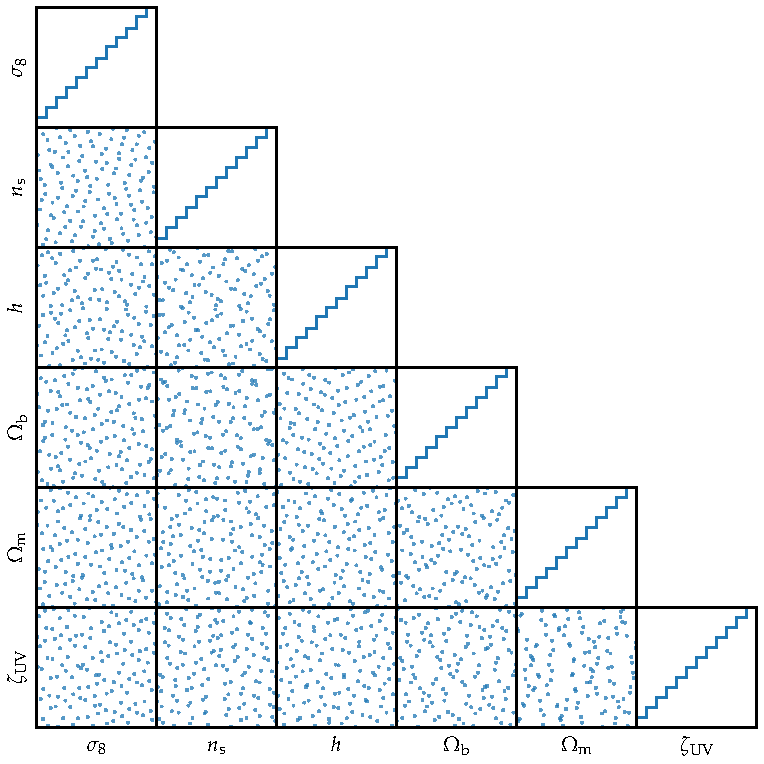
\includegraphics[width=25em]{figs/sobol128.pdf}
\caption{\textbf{Sobol sampling of our $x_\HI$ profiles}, in 6D
parameter space of $\sigma_8$, $\ns$, $h$, $\Omegab$, $\Omegam$, and
$\zetaUV$,
Each point in the lower triangular panels corresponds to the 2D
projection of a \texttt{21cmFAST} run, while the diagonal panels show
the 1D cumulative histograms for each parameter.
These 1D and 2D projections demonstrate the uniformity of our sampling
of the parameter space within the prior range of \cref{eq:prior}.}
\label{fig:sobol}
\end{figure}

The ionization efficiency $\zetaUV$ governs the ability of ultraviolet
photons to escape their parent galaxies and ionize the IGM. An increase
in $\zetaUV$ leads to an earlier completion of HI reionization.
Due to significant uncertainties surrounding $\zetaUV$, we opted to use
a constant value in each simulation.
Note that this choice was made for simplicity, and a more realistic
assumption could be that $\zetaUV$ is a function of halo mass
\cite{Park2019} or redshift.
However, our findings suggest that $\zetaUV$ plays a minor role compared
to the cosmological parameters.
In fact, the best performing symbolic regression expressions (see
\nameref{ssec:pysr} for the selection of best models) do not use
$\zetaUV$.


\subsection*{Helium reionization}
\label{ssec:helium}

The early intergalactic medium is primarily composed by neutral hydrogen
and helium.
Neutral helium (HeI) loses is first electron at the same time as neutral
hydrogen (HI) gets ionized \cite{Trac2007}.
However, there is a second reionization that occurs around $z\sim3$
where Helium (HeII) loses its remaining electron.

CMB photons will scatter off any free electrons, therefore both helium
reionizations contribute to the Thomson optical depth to reionization
$\tau_\reio$, although HeII ionization contribute relatively little in
comparison to HI and HeI ionizations \cite{Liu2016}.

To include the impact of the first helium reionization in our Gompertz
\texttt{CLASS}, we assume it follows that of HI as done in the $\tanh$
model, i.e.\ the free electron fraction $x_\e$ is given by
%
\begin{align}
\label{eq:xe_H_He}
x_\e
&= \Bigl(1 + \frac{n_\He}{n_\mathrm{H}} - x^\rec_\e\Bigr) x_\e^\gomp
  + x^\rec_\e
\nonumber\\
%
&= \Bigl(1 + \frac{Y_\He}{C (1 - Y_\He)} - x^\rec_\e\Bigr) x_\e^\gomp
  + x^\rec_\e,
\end{align}
%
where $n_\He / n_\mathrm{H}$ is the helium to hydrogen number density
ratio, $C \equiv m_\He / m_\mathrm{H} \approx 4$ is their mass ratio,
$Y_\He$ is the helium mass fraction, $x_\e^\gomp$ corresponds to the
contribution of free electrons due to \cref{eq:uni}, and $x^\rec_\e
\approx 10^{-4}$ is the leftover free electrons from after
recombination.

Given the relatively small impact of the HeII reionization on
$\tau_\reio$, the current uncertainties regarding its timeline, and the
difficulty involved with its accurate modeling \cite{Hotinli2023,
Upton2020}, we opt to follow the conventional approach and include the
second Helium reionization using the $\tanh$ model
%
\begin{equation}
\label{eq:xe_tot}
x_\e^\mathrm{Tot} = x_\e + \frac{Y_\He}{2C(1 - Y_\He)}
  \biggl(\tanh{\Bigl(\frac{z_\re^\HeII - z}{\Delta z^\HeII}\Bigr)} + 1\biggr),
\end{equation}
%
where $z_\re^\HeII = 3.5$ and $\Delta z^\HeII = 0.5$ are the midpoint
and duration of the second helium reionization, respectively.
These choices are also the default values used by \texttt{CLASS}.


\subsection*{Shape universality and modeling}
\label{ssec:shape}

\begin{figure}[tb]
\centering
\includegraphics[width=0.6\linewidth]{figs/shape_6.pdf}
\caption{\textbf{Universal shape of $x_\HI$.}
\emph{(Top)} 128 simulated $x_\HI$ timelines (thin light gray lines)
exhibit universality, after power-law transformations $\ar =
(a/\ap)^\tilt$.
The blue curves in all panels show our fitted analytic shape model, a
composition of the Gompertz curve with a 5th-degree polynomial in
\cref{eq:uni,eq:poly}.
\emph{(Middle)} Time derivative of $x_\HI$, can be interpreted as a PDF
if we view $x_\HI$ itself as the CDF.
We first discovered the universality by translating and rescaling each
$x_\HI$ using the mean and variance of its PDF, though now switch to the
better approach that jointly fits the global shape and individual
power-law parameters.
We use the latter as target of symbolic regression.
\emph{(Bottom)} Timelines transformed by the inverse of Gompertz
function, modeled in blue curve with a 5th-degree polynomial in
\cref{eq:poly}.}
\label{fig:shape}
\end{figure}

We discovered the universality in the shape of $x_\HI$ timelines before
attempting to build analytic model for it.
Because $x_\HI$ varies monotonically between 1 and 0, we can view it as
a CDF and derive its PDF, with which we can weigh the logarithmic scale
factor $\ln a$ to compute its mean and standard deviations.
It was immediately obvious to us that the $x_\HI$'s had a common shape
to percent level, after translation by their means and rescaling by
their standard deviations.
However, given our broad parameter range in \cref{eq:prior}, some
$x_\HI$'s have not reached 0 by the end of simulations, resulting in
imperfect transformations hurting the universality.

To address this, we construct flexible models for the universal shape,
and fit it jointly with individual transformation parameters of each
$x_\HI$ timeline.
We compose the Gompertz function $\gomp$, defined in \cref{eq:uni}, with
a low-degree polynomial $P_m$, where $m = 1, 3, 5, 7$ progressively.
We fit the composed shape to minimize the mean squared error (MSE) in
128 $x_\HI$'s and at 92 time points in each, and find the objective
value improve with $m$ but only marginally from $P_5$ to $P_7$.
Therefore, our final shape model is a composition of $\gomp$ and $P_5$,
(see the lower panel of \Cref{fig:shape}), and has 6 parameters to fit.

As for the transformation parameters, as in the PDF approach, we use an
affine transformation $\ln\ar = \tilt (\ln a - \ln\ap)$, or equivalently
a power law in \cref{eq:map}.
Because each $x_\HI$ has its own parameters of $\ap$ and $\tilt$, we
have in total $262 = 6 + 2 \times 128$ parameters to determine in the
joint fit.
\Cref{fig:shape} shows all 128 $x_\HI$ timelines and their universality
after transformations.
We can then use the fitted $\ap$ and $\tilt$ as the target for symbolic
regression, to model their cosmological dependences on the other
independent parameters.


\subsection*{Symbolic regression}
\label{ssec:pysr}

\begin{figure}[tb]
\centering
\includegraphics[width=0.8\linewidth]{figs/pareto.pdf}
\caption{\textbf{Pareto front for symbolic regression} (blue solid
steps) illustrates the trade-off between regression accuracy and
expression complexity.
We further add the lower convex hull to aid model selection: each
segment of the orange dotted line represents a power-law trade-off in
this log-log plot, and every model that touches the convex hull is more
economic -- in the sense of accuracy gain at cost of complexity -- than
the nearby models above the segments.
As an example, here we show the results of $\ln\ap(\vtheta)$, where the
complexity 11 point gives \cref{eq:SR}.}
\label{fig:pareto}
\end{figure}

SR learns from data using analytic expressions, unlike traditional
methods that adjust parameters in a fit.
Moreover, it can be employed to interpret deep neural network outputs
\cite{Cranmer2020b}.
\YLtodo[inline]{Miles, it'd be great if you can refine/rewrite the SR
and PySR intro}

With \texttt{PySR}, we search for symbolic expressions that take the 6
parameters in \Cref{fig:sobol} as inputs and output $\ln\ap$ or $\tilt$,
to minimize the MSE loss.
Here, the search space is the set of expressions composed of 5 binary
operators ($+$, $-$, $\cdot$, $/$, and power function) and 2 unary
operators ($\exp$ and $\ln$).
Each expression naturally takes the form of a binary tree, and the
total number of nodes is a measure of its complexity.

More complex expressions tend to fit more accurately, a trade-off
typically visualized by the Pareto front, as shown in \Cref{fig:pareto}.
Better and more economic expressions can achieve a lower loss at
moderate increase of complexity.
To aid model selection, we use a heuristic that compares all expressions
on the Pareto front globally, and only considers models that fare
favorably in power-law trade-offs of the form
%
\begin{equation}
\mathrm{loss}^{1 - \gamma} \cdot \mathrm{complexity}^\gamma
= \mathrm{const}, \quad \forall \gamma \in (0, 1).
\end{equation}
All such expressions lie on the lower convex hull of the Pareto front,
as illustrated in \Cref{fig:pareto}.

We use 512 populations each has 33 expressions, and we optimize for
10000 iterations and 10000 cycles in each.\YLtodo[inline]{Miles, could
you translate this into some brief description in the language of
evolve-simplify-optimize loop, mutation, crossover, and tournament?}

For the pivot $\ln\ap$, we find complexity 11 is enough for the MSE loss
to reach $10^{-4}$ (sub-percent level error on average), so there's no
need to use expressions more complex that that.
However, for the tilt $\tilt$, complexity 1, i.e.\ a constant, fit with
a loss $\approx 0.1$ ($4\%$ error on average), while higher complexities
can help but very slowly.
Therefore, based on the economic heuristic, we choose expressions of
complexity 11 and 1, for $\ln\ap$ and $\tilt$, respectively.

This preference for constant tilt could be a consequence of the
astrophysical assumptions of reionization in \texttt{21cmFAST}.
A more complex simulation, such as one involving radiative transfer or
different X-ray preheating \cite{Montero2024}, might reveal a different
tilt.

\begin{table}[t]
\centering
\caption{\textbf{Parameter constraints from Planck CMB data.}
Summary table of the constraints for representative parameters of the
universal shape (Gompertz) and $\tanh$ reionization models.
The constraints use CMB `TTTEEE' + lensing information.
The results from Planck analysis \cite{Planck2020a} are included for
comparison.
The validation models are gomp 0 and $\tanh$ 0, gomp 0 does not include
the cosmological information present in the timeline of reionization.
In contrast, gomp 1, and the alternative mapping gomp 2, both include
the additional cosmological dependence in the reionization timeline.
The shaded cells highlight the parameters that are sampled over by MCMC
for the different models.
\YL{The numbers in paretheses give the marginalized 1$\sigma$ uncertainty
in the last two significant digits.
We highlight the best constraints in boldface, by factors of 12 and 2.5
on $A_s$ and $\tau_\reio$, respectively.
The age of the Universe and $H_0$ are in unit of Gyr and km/s/Mpc,
respectively, and $S_8 \equiv \sigma_8 \sqrt{\Omegam/0.3}$ as usual.}}
\YLtodo[inline]{Should be say something about absence of $z_\re$ uncertainty?
Bold gomp 1 and gomp 2 look worse, better, or should I bold even more
derived params that improve?}
\makebox[\textwidth][c]{\footnotesize
\renewcommand{\arraystretch}{1.3}
\begin{tabular}{c *{3}{r} !{\hspace{.5em}} *{3}{r}}
\toprule
 & \multicolumn{3}{c}{Gompertz reionization} & \multicolumn{3}{c}{Tanh reionization} \\
\cmidrule(lr){2-4} \cmidrule(lr){5-7}
Parameter & gomp 0 & gomp 1 & gomp 2 & $\tanh$ 0 & $\tanh$ 1 & Planck PR3\cite{Planck2020a} \\
\midrule
$10^{9} \As$ & \sampled 2.101(31) & \textbf{2.088(12)} & \textbf{2.089(13)} & \sampled 2.099(30) & 2.098(30) & \sampled 2.100(30) \\
$\ns$ &\sampled 0.9638(41) & \sampled 0.9634(40) & \sampled 0.9634(40) & \sampled 0.9641(42) & \sampled 0.9641(41) & \sampled 0.9649(42) \\
$\Omegac h^2$ &\sampled 0.1201(12) & \sampled 0.1203(11) & \sampled 0.1202(11) & \sampled 0.1201(12) & \sampled 0.1201(12) & \sampled 0.1200(12) \\
$\Omegab h^2$ & \sampled 0.02235(15) & \sampled 0.02233(14) & \sampled 0.02233(14) &  \sampled 0.02235(15) & \sampled 0.02235(15) & \sampled 0.02237(15) \\
$\Omegam$ & 0.3157(76) & 0.3171(68) & 0.3168(68) & 0.3157(76) & 0.3159(75) & 0.3153(73) \\
$\Omegam h^2$ & 0.1430(11) & 0.1433(10) & 0.1432(10) & 0.1430(11) & 0.1431(11) & 0.1430(11) \\
$\OmegaL$ & 0.6842(76) & 0.6828(68) & 0.6831(68) & 0.6842(76) & 0.6840(75) & 0.6847(73) \\
Age & 13.800(23) & 13.803(20) & 13.803(22) & 13.800(23) & 13.800(23) & 13.797(23) \\
$H_0$ & 67.32(55) & \sampled 67.22(49) & \sampled 67.24(50) & 67.32(55) & \sampled 67.31(54) & 67.36(54) \\
$100 \theta_\mathrm{X}$ & \sampled 1.04184(29) & 1.04183(29) & 1.04183(29) & \sampled 1.04815(29) & 1.04184(29) & \sampled 1.04092(31) \\
$\sigma_8$ & 0.8109(59) & \sampled 0.8092(45) & \sampled 0.8092(46) & 0.8108(60) & \sampled 0.8105(59) & 0.8111(60) \\
$S_8$ & 0.832(13) & 0.832(13) & 0.832(13) & 0.832(13) & 0.832(13) & 0.832(13) \\
$\tau_\reio$ & \sampled 0.0546(76) & \textbf{0.05115(61)} & \textbf{0.05140(63)} & \sampled 0.0543(75) & 0.0538(74) & \sampled 0.0544(73) \\
$z_\re$ & 6.81(68) & 7.40 & 7.41 & 7.67(75) & \sampled 7.62(74) & 7.67(73) \\
\bottomrule
\end{tabular}}
\label{tab:uber-table}
\end{table}

\begin{figure}[tb]
\centering
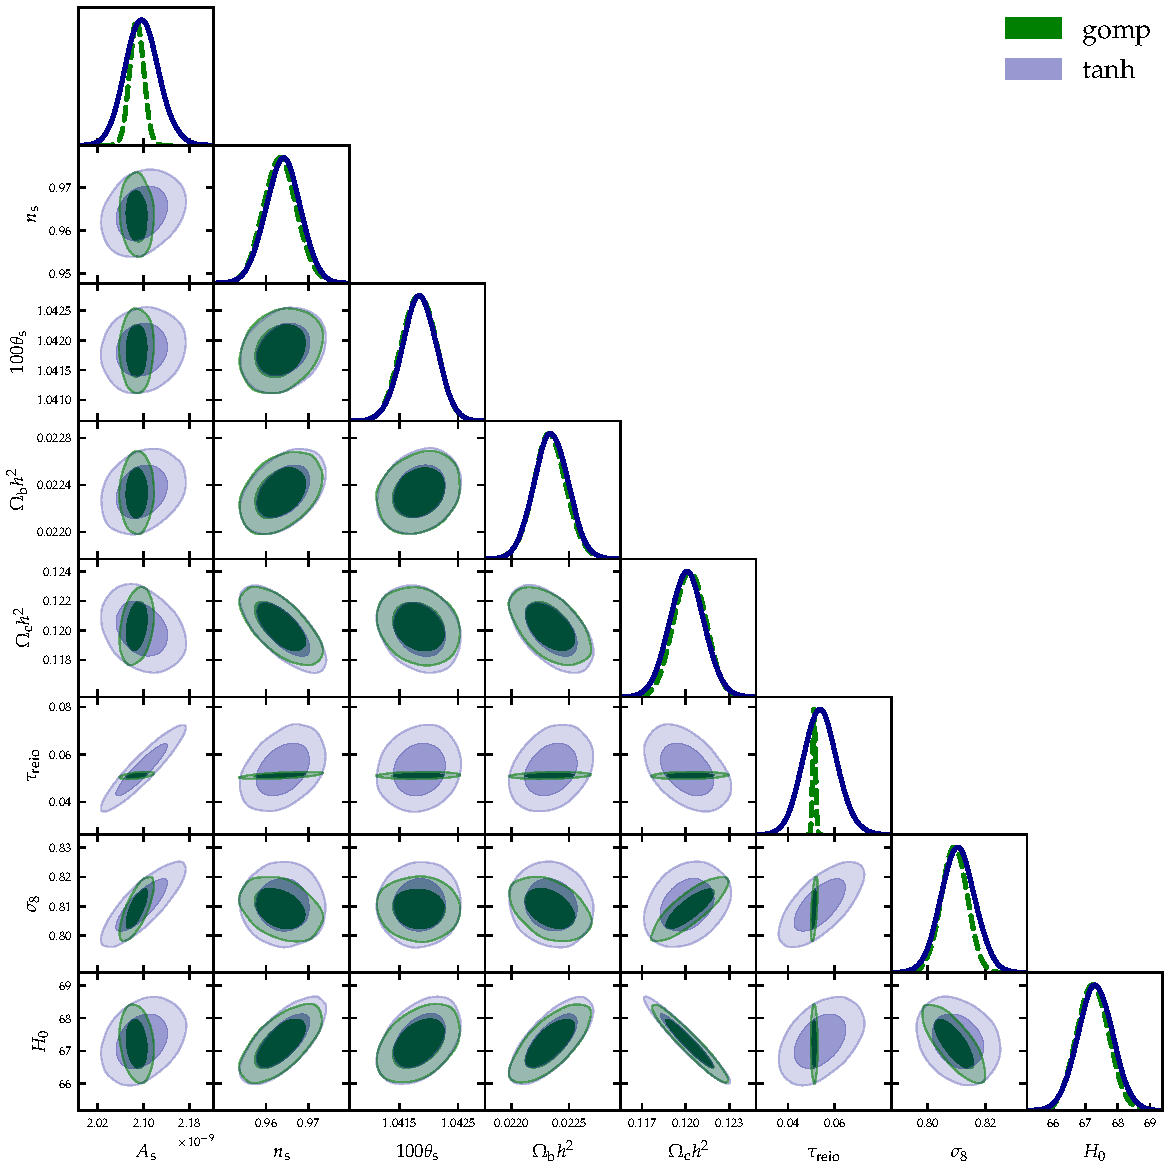
\includegraphics[width=\linewidth]{figs/gomp_tanh_triangle_kill_full.pdf}
\caption{\textbf{Analysis of CMB data treating $\tau_\reio$ as a derived
parameter using \cref{eq:uni,eq:poly,eq:map,eq:SR} vs.\ sampling it with
the conventional $\tanh$ model.} Here gomp 1 combines our Gompertz universal
shape with the rescaling pivot and tilt obtained via symbolic regression. Note that for
gomp 1 we do not sample over $z_\re$ since \cref{eq:uni} does not depend on it.
The green (blue) contours correspond to the constraints obtained with
our Gompertz universal shape ($\tanh$ 1 model).}
\label{fig:unleashed_gomp}
\end{figure}


\begin{figure}[tb]
\centering
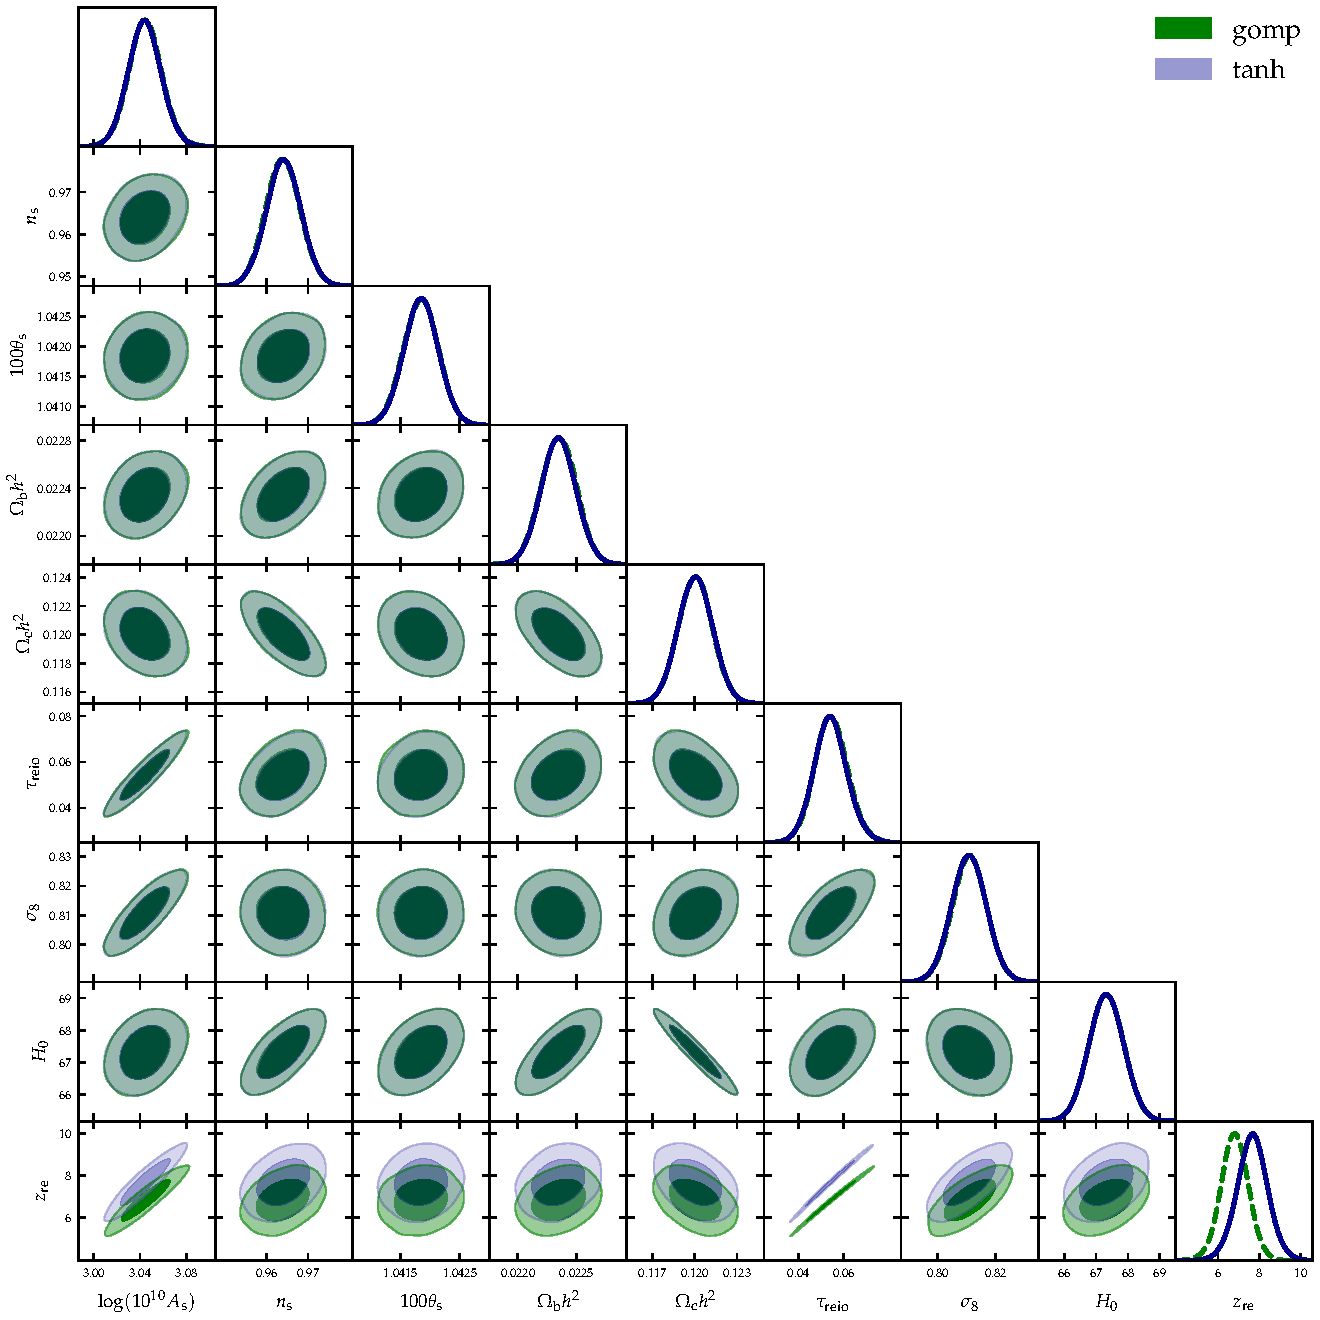
\includegraphics[width=\linewidth]{figs/gomp_tanh_triangle_tau.pdf}
\caption{\textbf{Validation of our universal shape for $x_\HI$ in \cref{eq:uni,eq:poly} vs.\ the
conventional $\tanh$ model using CMB data with sampling over $\tau_\reio$.}
Note that we have not \emph{eliminated} $\tau_\reio$ from the analysis
yet. Here, we use the standard choice of sampling
over optical depth and obtain the corresponding reionization history via bisection.
The green (blue) contours correspond to the constraints obtained with
our gomp 0 ($\tanh$ 0) model.}
\label{fig:tg}
\end{figure}

\subsection*{Alternative mapping}
\label{ssec:0226}

The mapping between neutral hydrogen profiles and cosmology is not
unique.
This is because symbolic regression algorithms can be non-convergent.
Moreover, the resulting symbolic expressions can depend on the data used
for training, i.e.\ overfitting.

To investigate the impact of overfitting, we train an alternative
mapping of reionization with cosmology using only half of the
\texttt{21cmFAST} $x_\HI$ profiles, which we refer as gomp 2.
For the tilt, once again we find a constant $\tilt = 8.331$, remarkably
close to the value obtained using the full simulated data (8.290).
And for the pivot, we obtain
%
\begin{equation}
\label{eq:SR0226}
\ln\ap(\vtheta) = (1.039 + \sigma_8) (\Omegab - \Omegam h - \ns),
\end{equation}
%
with a training loss of $1.2 \times 10^{-4}$.
Now we can test this on the other half of our $x_\HI$ sample and get a
validation loss of $1.4 \times 10^{-4}$, only slightly larger than the
training loss implying we are safe from overfitting.

Unsurprisingly, \cref{eq:SR0226} recovers the cosmological trends
present in \cref{eq:SR}.
Specifically, increasing $\ns$, $\Omegam$, and $\sigma_8$ leads to an
earlier reionization scenario, while a higher value of $\Omegab$
slightly delays reionization.
Furthermore, the impact of the Hubble constant is once again linked to
the matter density, albeit not in the same manner as in
\cref{eq:SR}.
This is likely evidence that the role of $h$ is limited, and
\texttt{PySR} considers its influence in conjunction with $\Omegam$
without increasing the complexity of the analytic expression.

Replacing \cref{eq:SR} with \cref{eq:SR0226}, we rerun the analysis
following the same approach, and summarize the results in
\Cref{tab:uber-table}.
Comparing these findings to our previous results, we observe strikingly
similar values for all cosmological parameters, albeit with smaller
deviations from the Planck results.
The consistency between our results using the full $x_\HI$ sample and
those using only half of it indicates that our symbolic expression
mappings perform robustly and are not biasing the parameter inferences.


\subsection*{MCMC inference}
\label{ssec:fits}

\Cref{tab:uber-table} summarizes the
results obtained by performing MCMC Bayesian inference with
\texttt{Cobaya} for the models considered throughout this work.
We also include the Planck results \cite{Planck2020a} for reference.
In total, we run three Gompertz reionization and two $\tanh$
reionization models, where $\tanh$ 0, Planck PR3, and gomp 0 sample over
the typical 6 cosmological parameters (see shaded parameters in
\Cref{tab:uber-table}).
In contrast, gomp 1, and gomp 2 sample over $\vtheta = \{\sigma_8, \ns,
\Omegab h^2, \Omegac h^2, h\}$.
Similarly, $\tanh$ 1 samples over the same parameters as gomp 1 but with
the inclusion of $z_\re$, and agrees with $\tanh$ 0 as the expected
result from this sanity check.

There is an apparent discrepancy between the different models in
$\theta_\mathrm{x}$, a proxy for the angular scale of the acoustic
oscillations ($\theta_*$).
The difference is due to our use of $100\theta_\mathrm{s}$, which
corresponds to the peak scale parameter defined exactly as the
ratio of the sound horizon divided by the angular diameter at
decoupling, with decoupling time given by the maximum of the visibility
function, i.e.\ the standard choice for CLASS.
In contrast, the Planck collaboration reports $100\theta_\mathrm{MC}$,
which is given by Eq.~(6) in \cite{Planck2014}, and corresponds to the
standard choice in \texttt{CosmoMC}\cite{Lewis2002}.
